\documentclass{article}
\usepackage{amsmath}
\usepackage{amsfonts}
\usepackage{tikz}
\usetikzlibrary{positioning}

\usepackage[shortlabels]{enumitem}

\usepackage{algorithm}
\usepackage{amssymb}
\usepackage{booktabs}
\usepackage{algpseudocode}

\textwidth=7.6in
\textheight=9.9in
\topmargin=-.9in
\headheight=0in
\headsep=.5in
\hoffset=-1.5in
\setlength\parindent{0pt}


\begin{document}

\begin{center}
    \Large{\textbf{Problem Set 1 Solutions}} \\[0.25ex]
    Calvin Walker
\end{center}
\textbf{1.}
\begin{enumerate}[(a)]
    \item \begin{enumerate}[(i)]
        \item \begin{align*}
            P(A|B, E)P(B | E) &= \frac{P(A, B, E)}{P(B, E)}P(B|E) = \frac{P(A, B, E)}{P(E)P(B|E)}P(B|E) \\[0.5ex]
            &= \frac{P(A, B, E)}{P(E)} = P(A, B | E)
        \end{align*}
        So $P(A, B | E) =  P(A|B, E)P(B | E)$ as needed. 
        \item \begin{align*}
            P(A|B,E) &= \frac{P(A, B, E)}{P(B, E)} = \frac{P(B|A,E)P(A|E)P(E)}{P(E)P(B|E)} \\[0.5ex]
            &= \frac{P(B|A,E)P(A|E)}{P(B|E)} 
        \end{align*}
    \end{enumerate}
    \item \begin{align*}
        P(X, Y | Z, W) &= \frac{P(X, Y, Z, W)}{P(Z, W)} = \frac{P(X, Y, W|Z)}{P(W | Z)} \\ 
        &= \frac{P(X|Z)P(Y, W|Z)}{P(W|Z)} \\
        &= P(X|Z)P(Y|Z,W)
    \end{align*}
    So $(X \perp Y|Z, W)$
    \item \begin{align*}
        P(X, Y, W | Z) &= P(X, W | Z, Y)P(Y | Z) \\ 
        &= P(X|Z, Y)P(W, Y | Z)P(Y|Z) = P(X|Z, Y)P(W, Y|Z) \\
        &= P(X|Z)P(W, Y|Z)
    \end{align*}
    So $(X \perp Y, W | Z)$
    \item \begin{enumerate}[(i)]
        \item \begin{align*}
            P(H|E_1, E_2) &= \frac{P(H, E_1, E_2)}{P(E_1, E_2)} = \frac{P(H)P(E_1|H)P(E_2|E_1, H)}{P(E_1, E_2)} \\
            &= \frac{P(H)P(E_1, E_2 | H)}{P(E_1, E_2)}
        \end{align*}
        So option $(b)$ is sufficient to compute $P(H|E_1, E_2)$
        \item If $(E_1 \perp E_2 | H)$, then: \begin{align*}
            \frac{P(H)P(E_1, E_2 | H)}{P(E_1, E_2)} &= \frac{P(H)P(E_1|H) P(E_2 | H)}{\sum_{i}P(E_1|H_i)P(E_2|H_i)}
        \end{align*}
        So option $(c)$ is sufficient to compute $P(H|E_1, E_2)$
    \end{enumerate}
    \item \begin{enumerate}[(i)]
        \item \begin{align*}
            E_p[-\log P(X)] &\leq \log E_p \bigg[ \frac{1}{P(X)} \bigg] \\[0.5ex]
            &= \log |\text{Val}(X)|
        \end{align*}
        \item \begin{align*}
            - E_p[- \log P(X)] &= - \sum_{X} P(X) (-\log P(X)) \\
            &= \sum_{X} P(X) \sum_{X} \log P(X) \\
            &\leq \log \sum_{X} P(X) = 0
        \end{align*}
        So $E_p[- \log P(X)] \geq 0$ as needed 
        \item \begin{align*}
            - E_p[\log \frac{P(X)}{Q(X)}] &= - \sum_X P(X) \log \frac{P(X)}{Q(X)} \\
            &= \sum_X P(X) \log \frac{Q(X)}{P(X)} \\
            &\leq \log \sum_X Q(X) = 0
        \end{align*}
        So $E_p[\log \frac{P(X)}{Q(X)}] \geq 0$ as needed 
    \end{enumerate}
    \item \begin{enumerate}[(i)]
        \item \begin{align*}
            H_p(X|Y) - H_p(X) &= E_p[-\log P(X|Y)] - E_p[-\log P(X)] \\ 
            &= E_p\bigg[\log \frac{P(X)}{P(X|Y)}\bigg] \\
            &= \sum_{X, Y} P(X, Y) \log \frac{P(X)}{P(X|Y)} = \sum_{X, Y} P(X, Y) \log \frac{P(X)}{P(X, Y)/P(Y)}\\
            &\leq \log \sum_{X,Y} P(X)P(Y) = 0
        \end{align*}
        So $H_p(X|Y) - H_p(X) \leq 0$ and $H_p(X|Y) \leq H_p(X)$ as needed 
        \item \begin{align*}
            -I(X;Y) &= -E_p\bigg[\log \frac{P(X|Y)}{P(X)}\bigg] \\
            &\leq -\log \sum_{X, Y} P(X, Y) \frac{P(X|Y)}{P(X)} = -\log \sum_{X, Y} P(X, Y)\frac{P(X,Y)/P(Y)}{P(X)} \\
            &= \log \sum_{X, Y}P(X)P(Y) = 0
        \end{align*}
        So $I(X;Y) \geq 0$ as needed
    \end{enumerate}
    \item  \begin{enumerate}[(i)]
        \item \begin{align*}
            I_p(X;Y|Z) &= E_p \bigg[ \log \frac{P(X|Y,Z)}{P(X|Z)}\bigg] \\[0.25ex]
            &= E_p [ \log P(X|Y,Z) - \log P(X|Z)] \\
            &= E[-\log P(X|Z)] - E_p[-\log P(X|Y,Z)] \\
            &= H_p(X|Z) - H_p(Z|Y,Z)
        \end{align*}
        \item \begin{align*}
            I_p(X;Y,Z) &= E_p\bigg[\log \frac{P(X|Y,Z)}{P(X)}\bigg] \\
            &= E_p[\log P(X|Y,Z) - \log P(X)] \pm  E_p[-\log P(X|Y)] \\
            &= E_p \bigg[\log \frac{P(X|Y)}{P(X)}\bigg] - E_p \bigg[\log \frac{P(X|Y,Z)}{P(X|Y)}\bigg] \\
            &= I_p(X;Y) + I_p(X;Z|Y)
        \end{align*}
    \end{enumerate}
\end{enumerate}
\textbf{2.1} \begin{enumerate}[(a)]
    \item No, there is an active trail $W \leftrightharpoons F \leftrightharpoons M$
    \item Yes, d-sep$(W, M | F)$ 
    \item No, there is an active trail $W \leftrightharpoons D \leftrightharpoons H$
    \item Yes, d-sep$(W, H | F, D)$
    \item No, there is an active trail $W \leftrightharpoons F \leftrightharpoons H \leftrightharpoons L \leftrightharpoons N$
    \item Yes, d-sep$(W, N | D, H)$
    \item No, $F$ and $D$ have a common cause $W$
    \item No, there is an active trail $F \leftrightharpoons H \leftrightharpoons D$
    \item Yes, d-sep$(F, D | W)$
    \item No, conditioning on $N$ activates the v-structure so there is an active trail $F \leftrightharpoons H \leftrightharpoons L \leftrightharpoons N \leftrightharpoons D$
    \item No, $M$ and $N$ share the common cause $F$
    \item No, there is an active trail $M \leftrightharpoons F \leftrightharpoons H \leftrightharpoons D \leftrightharpoons N$
\end{enumerate}
\textbf{2.2} : $P(W, F, D, M, H, L, N) = P(W)P(F|W)P(D|W)P(M|F)P(H|F,D)P(L|H)P(N|L,D)$ \\[1.5ex]
\textbf{2.3} \begin{enumerate}[(a)]
    \item $P(F) = P(F|W)P(W) + (F|\neg W)P(\neg W) = 0.25$
    \item $P(F|W, H) = \frac{P(F, W, H)}{P(W, H)} = \frac{\sum_D P(W, F, D, H)}{\sum_D \sum_F P(W, F, D, H)} = \frac{0.162}{0.267} = 0.61$
    \item $P(F|W, D, H) = \frac{P(F, W, D, H)}{P(W, D, H)} = 0.43$
\end{enumerate}
\textbf{3.} \begin{enumerate}[(a)]
    \item \begin{align*}
        P(H | V) &= \frac{P(V, H)}{\sum_h (V, h)} \\
        &= \frac{\exp(h^TWv + a^Tv + b^Th)/Z}{\sum_h \exp(h^TWv + a^Tv + b^Th)/Z} \\[0.5ex]
        &= \frac{\prod_j \exp(\sum_i h_j w_{ij}v_i + b_jh_j)}{\sum_{h} \prod_j \exp(\sum_i h_j w_{ij}v_i + b_jh_j)} \\[0.5ex]
        &= \frac{\prod_j \exp(\sum_i h_j w_{ij}v_i + b_jh_j)}{\prod_j \sum_{h_j \in \{0, 1\}}\exp(\sum_i h_j w_{ij}v_i + b_jh_j)} \\[0.5ex]
        &= \frac{\prod_j \exp(\sum_i h_j w_{ij}v_i + b_jh_j)}{\prod_j (1 + \exp(b_j + \sum_i w_{ij}v_i))} \\[0.5ex]
        &= \prod_j P(H_j | V)
    \end{align*}
    \begin{align*}
        P(H_j = 1 | V) &= \frac{\exp( b_j + \sum_i h_i w_{ij}v_i)}{(1 + \exp(b_j + \sum_i w_{ij}))} \\[0.5ex]
        &= \sigma(b_j + \sum_{i} w_{ij}v_i)
    \end{align*}
    \item \begin{align*}
        P(V | H) &= \frac{P(V, H)}{\sum_v (v, H)} \\
        &= \frac{\exp(h^TWv + a^Tv + b^Th)/Z}{\sum_v \exp(h^TWv + a^Tv + b^Th)/Z} \\[0.5ex]
        &= \frac{\prod_i \exp(\sum_j h_j w_{ij}v_i + a_iv_i)}{\sum_{h} \prod_i \exp(\sum_j h_j w_{ij}v_i + a_iv_i)} \\[0.5ex]
        &= \frac{\prod_i \exp(\sum_j h_j w_{ij}v_i + a_iv_i)}{\prod_i \sum_{v_i \in \{0, 1\}}\exp(\sum_j h_j w_{ij}v_i + a_iv_i)} \\[0.5ex]
        &= \frac{\prod_i \exp(\sum_j h_j w_{ij}v_i + a_iv_i)}{\prod_i (1 + \exp(a_i + \sum_j h_jw_{ij}))} \\[0.5ex]
        &= \prod_i P(V_i| H)
    \end{align*}
    \begin{align*}
        P(V_i = 1 | H) &= \frac{\exp(a_i + \sum_j h_i w_{ij}v_i)}{(1 + \exp(a_i + \sum_j h_jw_{ij}))} \\[0.5ex]
        &= \sigma(a_i + \sum_{j} h_jw_{ij})
    \end{align*}
    \item Yes, as shown in parts (a) and (b), the hidden units are conditionally independent given the visible units and vice versa. So the Markov network is an I-map for the distribution in Equation 2.
    \item \begin{align*}
        \frac{\partial \log P(V = v)}{\partial w_{ij}} &= \frac{\partial}{\partial w_{ij}} \log \frac{1}{Z}\sum_{h}\exp(-E(v, h)) \\[0.5ex] 
        &= \frac{\partial}{\partial w_{ij}} \log \sum_{h} \exp(-E(v, h)) - \frac{\partial}{\partial w_{ij}} \log Z \\[0.5ex]
        &= \frac{\frac{\partial}{\partial w_{ij}}\sum_h \exp(-E(v, h))}{\sum_h \exp(-E(v,h))} - \frac{\frac{\partial}{\partial w_{ij}} Z}{Z} \\[0.5ex]
        &= \frac{\sum_h \exp(-E(v, h))\frac{\partial}{\partial w_{ij}}(-E(v, h))}{\sum_h \exp(-E(v, h))} - \frac{\sum_{v, h}\exp(-E(v,h))\frac{\partial}{\partial w_{ij}}(-E(v,h))}{Z} \\[0.5ex]
    \end{align*}
    Where $\frac{\partial}{\partial w_{ij}}(-E(v, h)) = v_ih_j$. So 
    \begin{align*}
       & \frac{\sum_h  \exp(-E(v, h))\frac{\partial}{\partial w_{ij}}(-E(v, h))}{\sum_h \exp(-E(v, h))} - \frac{\sum_{v, h}\exp(-E(v,h))\frac{\partial}{\partial w_{ij}}(-E(v,h))}{Z} \\[0.5ex]
       &=  \sum_h P(H = h|V = v)v_ih_j - \sum_{v,h}P(V = v, H = h)v_ih_j \\[0.5ex]
       &= \mathbb{E}[V_iH_j|V = v] - \mathbb{E}[V_iH_j]
    \end{align*}
    \item $w_{00}, w_{10}, w_{20}$ and $w_{30}$ would be positive as all the films are in the action drama except ``The Notebook''. Similarly, $w_{11}$ and $w_{41}$ would be positive since ``Casablanca'' and ``The Notebook'' are in the romance genre.
\end{enumerate}
\textbf{4.} \begin{enumerate}[(a)]
    \item 
    \item For all $(X \perp Y\ |\ MB_H(X))$, $Y \notin MB_H(X)$ and $X \notin MB_H(Y)$, so $X - Y \notin H$ and thus $(X \perp Y\ |\ \mathbf{X} - \{X, Y \})$. So if $P \vDash I_{l}(H)$, then $P \vDash I_{p}(H)$.
    \item \begin{enumerate}[(i)]
        \item Let $U_1$ and $U_2$ be sets in $\mathcal{U}$. Then, \begin{align*}
            P \vDash (X \perp U_2 - U^*, \mathbf{X} - \{X\} - U^*\ |\ U_1 - U^*, U^*)\ \&  \ (X \perp U_1 - U^*, \mathbf{X} - \{X\} - U^*\ |\ U_2 - U^*, U^*)
        \end{align*}
        So by intersection and decomposition \begin{align*}
            P \vDash (X \perp U_1 - U^*, U_2 - U^* \ |\ U^*)
        \end{align*}
        Combining the results \begin{align*}
            P \vDash (X \perp U_1 - U^*, U_2 - U^*, \mathbf{X} - \{X\} - \{U_1, U_2\}\ |\ U^*)
        \end{align*}
        So $P \vDash (X \perp \mathbf{X} - \{X\} - U^*\ | \ U^*)$, and $U^* \in \mathcal{U}$. By definition, $MB_P(X)$ is the minimal set $U \in \mathcal{U}$, which is $U^*$. 
        \item \begin{align*}
            P &\vDash (X \perp Y | \mathbf{X} - \{X, Y\}) \\
            P &\vDash (X \perp \mathbf{X} - \{X\} - (\mathbf{X} - \{X, Y\}) | \mathbf{X} - \{X, Y\})
        \end{align*} 
        So $P \vDash (X \perp \mathbf{X} - \{X\} - U |\ U)$. But, $Y \notin U$ so $Y \notin U^* =  MB_P(X)$
        \item If $Y \notin MB_P(X)$ then $Y \in \mathbf{X} - \{X\} - MB_P(X)$ and $(X \perp Y, \mathbf{X} - \{X, Y\} - MB_P(X)\ |\ MB_P(X) )$. By weak union, $(X \perp Y\ |\mathbf{X} - \{X, Y\} - MB_P(X), MB_P(X))$. Thus, $(X \perp Y\ |\ \mathbf{X} - \{X, Y\})$
        \item Parts (ii) and (iii) demonstrate that $MB_P(X)$ is exactly the set of neighbors of $X$ in $H$, and thus a minimal I-map for $P$.
    \end{enumerate}
\end{enumerate}
\textbf{5.} \begin{enumerate}[(a)]
    \item \textcolor{white}{{s}}\begin{center}
        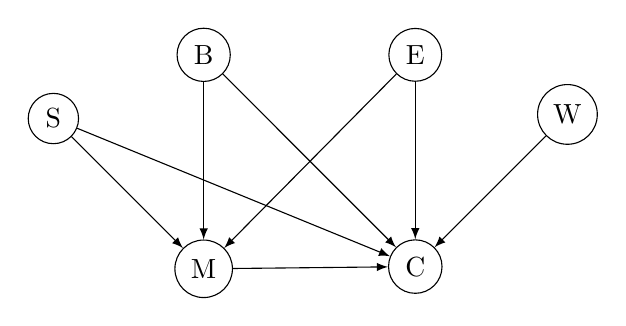
\begin{tikzpicture}[node distance=2.0cm]
            % Nodes
            \node[draw, circle] (B) {B};
            \node[draw, circle, right=of B] (E) {E};
            \node[draw, circle, below=of E] (C) {C};
            \node[draw, circle, below=of B] (M) {M};
            \node[draw, circle, above left=of M] (S) {S};
            \node[draw, circle, above right=of C] (W) {W};
    
            % Edges
            % \draw[-latex] (B) -- (E);
            \draw[-latex] (E) -- (C);
            \draw[-latex] (B) -- (M);
            \draw[-latex] (S) -- (M);
            \draw[-latex] (S) -- (C);
            \draw[-latex] (M) -- (C);
            \draw[-latex] (W) -- (C);
            \draw[-latex] (E) -- (M);
            \draw[-latex] (B) -- (C);

        \end{tikzpicture}
    \end{center}
    The above Bayesian Network is a minimal I-map for the marginal distribution over the remaining variables. When removing $A$ from the original network, we preserve the active trails from $B$ and $E$ to $M$ and $C$ that previously passed through $A$. Furthermore, in the original network, if conditioning on $M$, due to the v-structure, there was a dependency between $S$ and $C$ (the symmetric dependency between $W$ and $M$ when conditioning on $C$ is also preserved with this edge). The dependency between $M$ and $C$ (common cause $A$) in the orginal network is preserved without loss of generality by a new edge from $M$ to $C$. 
    \item We can generalize the above process as follows. When removing $X_i$, for each child of $X_i$ in $BN$, we add edges from the parents of $X_i$, an edge from the other decendents of $X_i$, and an edge from the parents of the other children of $X_i$. Formally, let Pa$_{X_j}'$ denote the parents of $X_j$ in $BN'$. For each child $X_j \in \text{Children}_{X_i}$ \begin{equation*}
        \text{Pa}_{X_j}' = \text{Pa}_{X_j} \cup \text{Pa}_{X_i} \cup \{X_k, \text{Pa}_{X_k} | X_k \in \text{Children}_{X_i}, X_j \notin \text{Pa}'_{X_k}\}
    \end{equation*}
    Where the last condition prevents adding redundant dependencies as the algorithm progresses, for instance, over a topological ordering of $BN$. For non-children of $X_i$ in $BN$, $\text{Pa}_{X_j}' = \text{Pa}_{X_j}$. 
\end{enumerate}
\textbf{6.} \begin{enumerate}[(a)]
    \item I did not collaborate 
    \item 
\end{enumerate}
\end{document}
